
\clearpage
\cleardoublepage

\chapter{Datasets}
\label{chap:dataset}

The data used for experimentation is taken from \cite{willi_rath_2023_7779883} which contains different climate features. The data is generated by the simulations, these simulations are provided by the robust climate Earth models \cite{willi_rath_2023_7779883}.

The dataset provides multiple features which are listed below:
\begin{itemize}
    \item Sea Surface Temperature
    \item Surface Air Temperature
    \item Sea Level Pressure
    \item Sea Surface Salinity
    \item Geopotential Height (500mb)
    \item Precipitation
\end{itemize}

The features that we considered for the experimentation were the geopotential height and precipitation.
Both of the datasets are timeseries data, where measurement for each feature is done by month for a 1000 year. Each of the datasets are explained in detail for the better understanding of the dataset.
\subsection{Geopotential Height Dataset}
It consists of 12000 geo referenced data points, where each geo referenced data point is a grid of (96x192) containing geopotential height value specific to a pair latitude and longitude.
Each geo referenced data point does also contains a time value associated with it as well.

96  is the total number of latitude values and  192 is the total number of longitude values, against which feature data is generated. The total number of geopotential height measurements for each month is 18816.

\begin{figure}[H]
    \centering
    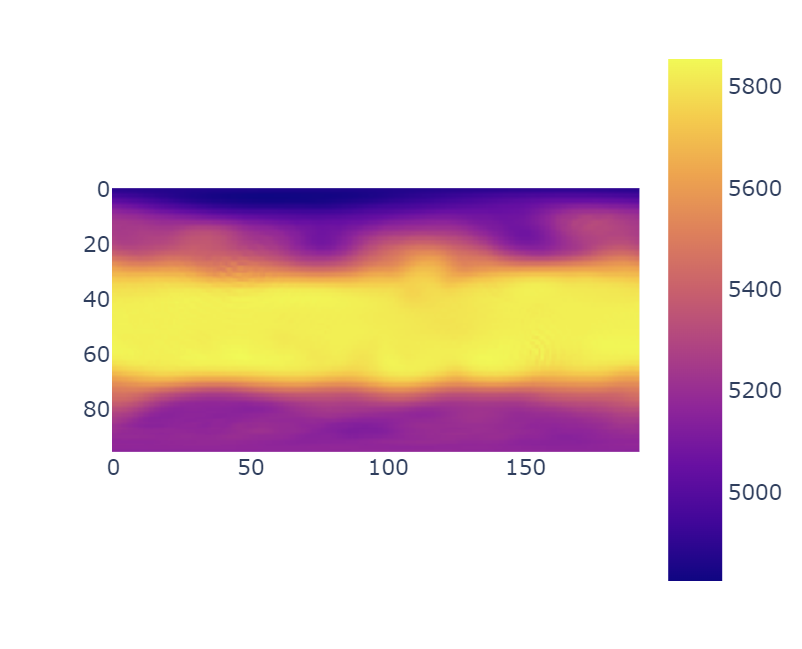
\includegraphics[width=0.6\linewidth]{figures/chapter-5/data_original.png}
    \caption{Original Geopotential Height 96x192 Grid }
    \label{fig:org_geopoth}
\end{figure}

\subsection{Precipitation Dataset}

The dataset for precipitation, which is geographically referenced, comprises 11988 data points. These points are organized as a grid of dimensions (96x144). The simulation generates data for a span of 999 years. Each index in the 2d array represents a geo-referenced observation of precipitation. The grid points are referenced using latitudes and longitudes.
Each grid of data is also associated to a month of the year.

96 is the total number of latitude values and 144 is the total number of longitude values. The total number precipitation measurement globally are 13824, means each grid contains the 13824 points in total.

\begin{figure}[H]
    \centering
    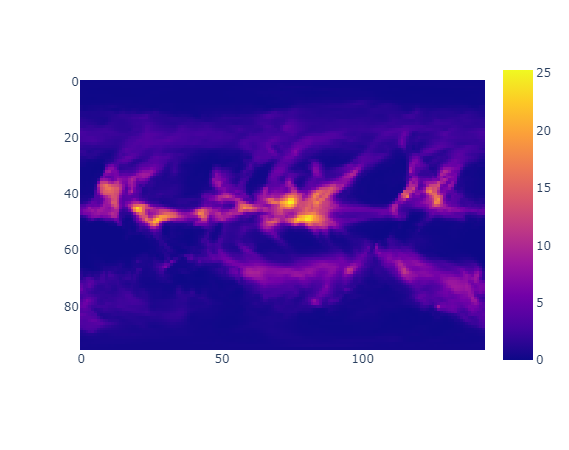
\includegraphics[width=0.6\linewidth]{figures/chapter-5/precipitation_raster.png}
    \caption{Original Precipitation 96x144 Grid }
    \label{fig:org_geopoth}
\end{figure}